Ao refletir sobre esse estudo, nos deparamos de volta com um panorama onde a observação fenomenológica se encontra com a tecnificação das mãos — um domínio onde a interação humana e a análise computacional convergem. Por um lado, a rede social Colab desdobra-se como um campo fértil onde as opiniões e estímulos dos usuários dispersam-se, dando vida a padrões de engajamento e ressonância. Por outro, nós, os pesquisadores, emergimos não apenas como observadores, mas como participantes ativos na interpretação dessa realidade, empregando a tecnologia para desvendar os fenômenos subjacentes às interações dos usuários. O desafio e, simultaneamente, o potencial dessa abordagem, residem na capacidade de compreender as múltiplas facetas da experiência digital e seu impacto sobre a esfera pública.

A proposta desse estudo foi sempre de tentar alcançar um passo além da análise de dados; nós procuramos compreender as dinâmicas ocultas que configuram o diálogo cívico, as correntes de opinião que direcionam decisões coletivas e a dinâmica da participação política no contexto digital. O empenho em cartografar as câmaras de eco e os comportamentos polarizadores reflete uma imersão profunda na complexidade das interações sociais, evidenciando como essas estruturas virtuais refletem e, em alguns casos, intensificam as divisões presentes no nosso contexto político e social.

Os efeitos desses fenômenos são variados: no contexto cívico, percebe-se que as câmaras de eco podem tanto cristalizar o debate público quanto estimular a ação coletiva. No plano governamental, as percepções advindas desta análise fornecem ferramentas para desfazer nós de polarização e fomentar um diálogo mais abrangente e produtivo. De forma mais geral, os resultados desta pesquisa apontam para vias de fortalecimento de uma prática democrática mais sólida e aberta, que valorize e promova a diversidade de perspectivas.

Essa reflexão também nos leva a pensar sobre a relevância de examinar não só os dados que circulam pelas redes, mas também as ferramentas que nos capacitam a realizar tal exame. A instrumentalização tecnológica que guiou nossa pesquisa é, afinal, um espelho do fenômeno que buscávamos compreender — um atestado da relação contínua e reveladora entre a tecnologia e a vivência humana, uma conexão que persiste em evoluir e nos surpreender.

Na simbiose entre técnica e percepção, as heurísticas e ferramentas de software desenvolvidas revelaram-se como prismas, por meio dos quais nossa investigação ganhou profundidade. Reconhecendo a ausência de fórmulas definitivas para decifrar ecossistemas tão complexos quanto câmaras de eco ou prever o comportamento dos usuários, abraçamos heurísticas — atalhos pragmáticos que, mesmo sem garantir precisão absoluta, nos guiam a descobertas significativas em um terreno inexplorado.

Neste contexto, a fenomenologia nos orienta a enxergar o usuário não como um mero participante, mas como um agente de transformação. Este olhar repercute em duas vertentes: distorce, inevitavelmente, nossa interpretação do usuário no mundo real e recalibra a maneira como construímos e compreendemos as simulações computacionais. Assim, o usuário se revela como uma força viva, dinâmica, que atua e é atuada pelo tecido social do qual é parte integrante, tanto no ambiente virtual do Colab quanto nas modelagens que visam replicar a complexidade de suas interações sociais digitais. Sob essa perspectiva, voltamos agora o olhar para os resultados concretizados — frutos dos objetivos traçados no início desta pesquisa.

\section{Síntese dos Resultados Alcançados}

\subsection*{Objetivo Geral}
O desenvolvimento e a aplicação de um conjunto de métricas quantitativas resultaram na previsão efetiva de comportamentos polarizadores e na identificação de câmaras de eco dentro de comunidades da rede social Colab. A aplicabilidade das métricas foi comprovada em um ambiente de estudo de caso, proporcionando insights valiosos sobre a dinâmica de interação digital.

\subsection*{Objetivos Específicos}

\begin{itemize}
	\item \textbf{Análise das Interações dos Usuários:}
	      A investigação das interações dos usuários no aplicativo Colab elucidou que as cidades de Niterói, Santo André e Mesquita apresentavam maior atividade na plataforma. Esta descoberta orientou a condução subsequente da pesquisa e delineou o escopo para análises mais aprofundadas.

	\item \textbf{Análise Exploratória com Gephi:}
	      A exploração da rede realizada com o auxílio da ferramenta Gephi cumpriu múltiplos propósitos: confirmou a existência de múltiplas comunidades por meio de métricas de modularidade, validando a premissa que a rede do Colab é de fato composto por comunidades em vez de se apresentar como uma rede difusa. A exploração também ajudou a extrair as comunidades específicas das cidades em foco e, mediante técnicas de refinamento de dados e filtragem, isolou os nós e comunidades centrais, otimizando a clareza analítica dos próximos passos.

	\item \textbf{Análise de Sentimento:}
	      O modelo desenvolvido para a classificação do sentimento das postagens demonstrou eficácia ao atribuir pontuações sentimentais numa escala de -1 a 1, baseando-se em postagens previamente categorizadas, obtidas através de métodos de análise de linguagem natural.

	\item \textbf{Classificação de Personas de Usuários:}
	      A categorização dos usuários em personas emergiu da observação de padrões comportamentais, delineando perfis colaborativos e individualistas. A criação e aplicação do modelo de classificação, um Ensamble de Votação, permitiu a categorização precisa das postagens, culminando na definição de perfis dos usuários baseados em suas interações.

	\item \textbf{Análise de Eventos e Pressão Social:}
	      A análise dos eventos classificados por tipo e sua relação com as métricas de sentimento e personas ofereceu uma nova perspectiva sobre a pressão social exercida nas cidades estudadas. O Colab se revelou um barômetro social hiperlocal, permitindo a aferição do impacto social de eventos específicos e fornecendo uma visão detalhada sobre a dinâmica urbana.

	\item \textbf{Heurísticas para Detecção de Câmaras de Eco:}
	      A integração de técnicas analíticas avançadas resultou na formulação de um teorema matemático destinado a identificar comunidades com elevado grau de polaridade e tendência à formação de câmaras de eco.

	\item \textbf{Aplicação do Detector de Câmaras de Eco:}
	      A execução do modelo nas redes das três cidades com mais interações no Colab revelou a presença de câmaras de eco em diferentes magnitudes, com uma identificada em Niterói, cinco em Santo André e oito em Mesquita, sugerindo variações significativas na dinâmica social entre as localidades.

\end{itemize}

\section{Aprendizados da Pesquisa}

Nesta seção, sintetizamos os aprendizados chave obtidos durante a pesquisa, enfatizando as contribuições metodológicas e as implicações práticas para o entendimento e a gestão de dinâmicas sociais em plataformas digitais.

\subsection*{Integração de Análise de Redes e Sentimentos}

A pesquisa demonstrou que a combinação de análises de rede e sentimentos é uma estratégia eficaz para desenvolver métricas derivadas capazes de antecipar tendências de polarização tanto ao analisar os nós da rede em relação com os outros nós, quanto ao analisar o conteúdo gerado pelos usuários em relação ao conteúdo interagido pelos usuários. Esta abordagem analítica avançada, ao entrelaçar métricas comportamentais com avaliações qualitativas de conteúdo, informou nossa metodologia sobre a probabilidade de formação de câmaras de eco e a intensidade da polarização nas redes.

\subsection*{Aplicação de heurísticas derivadas de simulações em uma Rede Social Real}

Esta pesquisa propõe um avanço significativo na análise de redes sociais, aplicando diretamente as heurísticas desenvolvidas por \citeonline{2023_Atiqi_BOOK}, obtidas a partir de suas simulações de redes sociais utilizando a modelagem baseada em agentes, no contexto real da plataforma Colab. Ao integrar estas heurísticas, como ECC (Echo Chamber Coefficient) e GEC (Global Echo Chamber), foi possível analisar a dinâmica de opiniões e a formação de câmaras de eco entre os usuários do Colab. Esta abordagem, portanto, demonstrou a viabilidade de aplicar heurísticas derivadas de simulações em redes sociais reais, abrindo caminho para novas pesquisas que explorem a aplicabilidade de outras heurísticas em contextos similares.

As heurísticas de \citeonline{2023_Atiqi_BOOK} foram aplicadas para avaliar a polarização e a presença de câmaras de eco no Colab. Utilizando análise de sentimento, cada postagem dos usuários foi categorizada para determinar a polaridade da opinião. Estes dados, juntamente com informações sobre a interação dos usuários na rede, foram inseridos nas fórmulas de ECC e GEC e outras heurísticas propostas por Atiqi.

A aplicação das heurísticas revelou padrões de polarização e formação de câmaras de eco na rede social Colab. Os resultados obtidos validaram a eficácia das heurísticas de Atiqi em um contexto real, demonstrando que as métricas desenvolvidas a partir de simulações podem ser efetivamente utilizadas para analisar e entender fenômenos sociais em plataformas digitais autênticas.

\begin{enumerate}
	\item Validação Prática: A eficácia das heurísticas de Atiqi, originalmente derivadas de simulações, foi comprovada em um ambiente real de rede social. Isso fortalece a ponte entre teorias de simulação e sua aplicação prática em cenários reais.
	\item Ferramentas Analíticas Robustas: Ao aplicar essas heurísticas em dados reais, a pesquisa forneceu ferramentas analíticas robustas para identificar e compreender a formação de câmaras de eco e polarização em redes sociais.
	\item Orientações para Intervenções: Os insights gerados oferecem orientações valiosas para intervenções específicas que podem ser implementadas para mitigar os efeitos da polarização e promover a diversidade de opiniões.
\end{enumerate}

\subsubsection*{Desafios e Direções Futuras}

Apesar dos resultados promissores, a aplicação de heurísticas baseadas em simulação em ambientes reais também revela desafios, como a necessidade de adaptar e refinar continuamente essas heurísticas para capturar a complexidade e a evolução das dinâmicas sociais nas redes. Pesquisas futuras podem se concentrar em aprimorar essas heurísticas e explorar novas formas de aplicá-las em diferentes contextos de redes sociais.

A aplicação das heurísticas de Atiqi no Colab demonstra como as teorias e métodos desenvolvidos em ambientes simulados podem ser efetivamente transferidos para analisar fenômenos sociais em plataformas de redes sociais reais. Esta pesquisa não apenas valida importantes conceitos teóricos, mas também abre caminho para futuras investigações e aplicações práticas na análise de redes sociais. Representa um exemplo eloquente de como a pesquisa acadêmica pode ser diretamente aplicada para gerar insights valiosos em cenários do mundo real.

\subsection*{O Colab como Barômetro Social}

Interpretar o Colab como um barômetro social hiperlocal informa nossa metodologia sobre a dinâmica de câmaras de eco. Além disso, esta análise oferece uma perspectiva inestimável que pode ser valiosa para os stakeholders e administradores públicos, auxiliando na tomada de decisões informadas e no desenvolvimento de políticas públicas mais eficazes.

\subsection*{Polarização em Plataformas de Cidadania Digital}

A aplicação do modelo de detecção de câmaras de eco nas redes de Niterói, Santo André e Mesquita constatou que, mesmo em redes sociais com especializadas em cidadania como o Colab, não há imunidade contra elementos e agentes polarizadores. Tópicos como impostos, eleições, penalidades de tráfego e gentrificação surgem como áreas de pressão social significativa, sublinhando a necessidade de uma análise cuidadosa das interações e conteúdo gerado pelos usuários.

\subsection*{Pipelines para Análise de Redes}

Ao considerarmos a complexidade inerente ao gerenciamento de informações em plataformas digitais, torna-se imperativo estabelecer diretrizes estratégicas que norteiem os administradores do Colab na coleta, tratamento e análise de dados. As diretrizes sugeridas neste estudo são concebidas com o intuito de elaborar pipelines analíticos avançados. Estes visam não somente o monitoramento acurado da pressão social hiperlocal, mas também a identificação e o entendimento das dinâmicas que conduzem à formação de câmaras de eco, operando em tempo real. A implementação dessas recomendações detém a capacidade de revolucionar a utilização das informações recolhidas, favorecendo respostas mais eficientes aos desafios cívicos e, consequentemente, reforçando os pilares de práticas democráticas inclusivas e resilientes.

Em diálogos exploratórios com a equipe do Colab, desenvolvemos o Data Product Canvas, uma ferramenta metodológica que se integra ao arsenal de recursos empregados para a concepção de um sistema eficaz de detecção de câmaras de eco. O canvas, delineado de maneira a proporcionar uma visão estruturada e coesa, serve de alicerce para a compreensão dos requisitos intrínsecos ao aplicativo, bem como para a definição dos elementos cruciais que permeiam seu design e funcionalidades.

\begin{figure}[H]
	\centering
	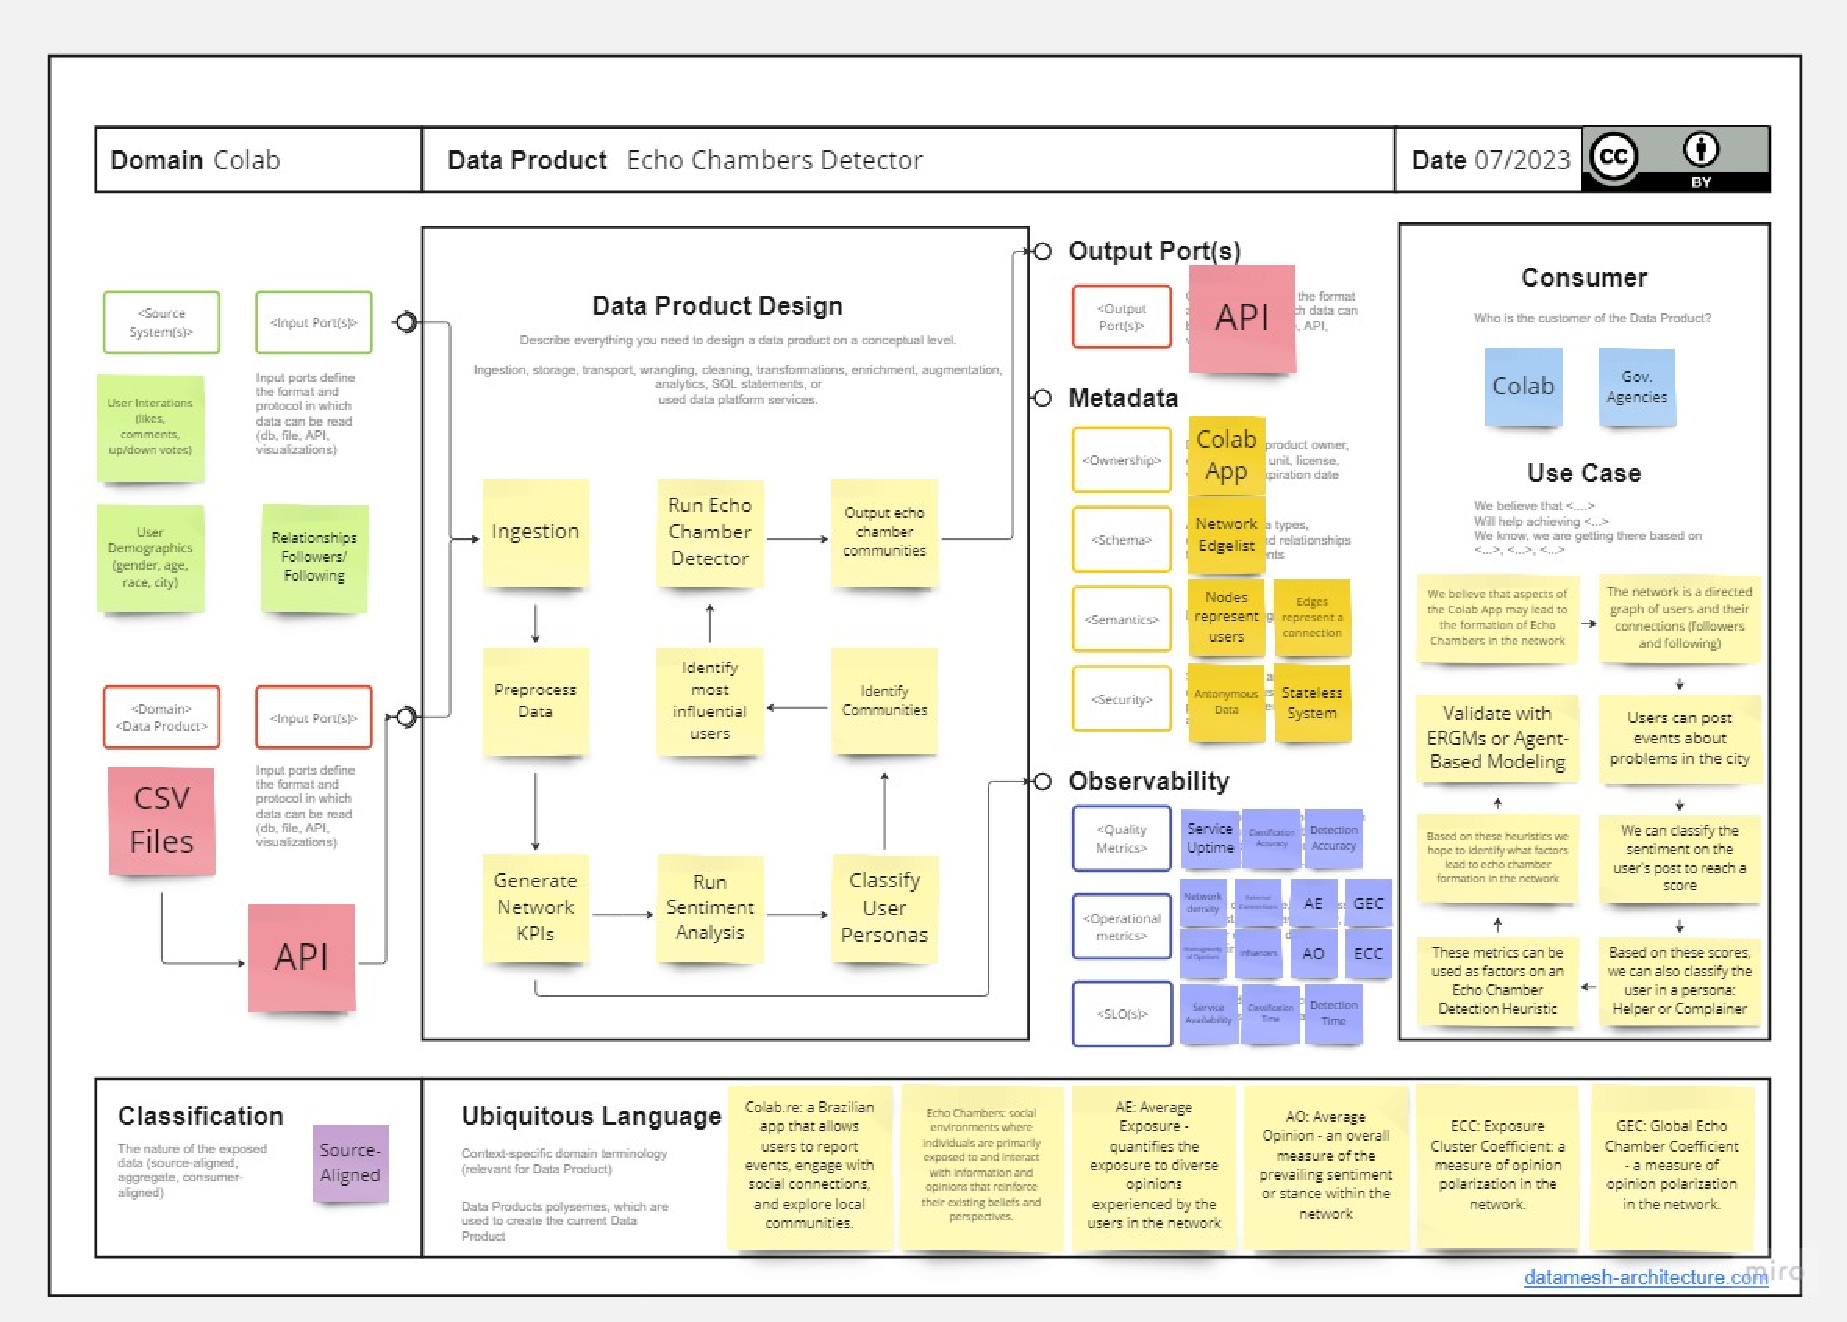
\includegraphics[width=0.9\textwidth]{tex/includes/data_canvas.pdf}
	\caption{Data Product Canvas desenvolvido para a estruturação do sistema de detecção de câmaras de eco.}
	\label{fig:data_canvas}
\end{figure}

Este instrumento emerge como um componente fundamental na aplicação das heurísticas de detecção de câmaras de eco em tempo real. O sistema concebido com base nesse canvas tem o potencial de fornecer alertas proativos aos administradores do Colab sobre emergentes câmaras de eco e tendências de polarização em tópicos específicos. A identificação precoce de tais fenômenos permite que os administradores adotem medidas preventivas e corretivas. Estratégias possíveis incluem a criação de novas categorias para postagens, a promoção de contribuições oriundas de perfis de usuários variados e a iniciação de tópicos de discussão inovadores, todos com o objetivo de mitigar a polarização e enaltecer a diversidade de opiniões dentro do ecossistema digital.

\subsection*{Validação de Conteúdo e a Gestão de Polarização nas Redes}

Ao discutir a implementação das heurísticas desenvolvidas em nesse estudo em sistemas de informação integrados ao Colab e num cenário onde sistemas automatizados ganham cada vez mais espaço na análise de interações em redes sociais, a reflexão sobre os mecanismos de moderação de conteúdo torna-se crucial. O desenvolvimento de métricas quantitativas e heurísticas para a identificação de indícios de polarização em redes digitais carrega consigo uma responsabilidade significativa. O objetivo primário de sistemas baseados nas heuristicas desse estudo deve ser a melhoria contínua dos serviços prestados pelo poder público nas cidades e o aprimoramento das plataformas de cidadania ativa, como o Colab.

As heurísticas de detecção de câmaras de eco e a análise de conteúdo postado pelos usuários, embora sofisticadas e valiosas, não podem operar isoladamente como juízes finais do que é considerado conteúdo polarizado. É imperativo que haja uma intervenção humana criteriosa, que atue como uma camada de validação final. Isto não apenas assegura a precisão e a relevância das conclusões do sistema, mas também protege contra a aplicação arbitrária de penalidades ou a remoção injustificada de conteúdo.

Por exemplo, a aplicação de punições ou a remoção de conteúdos baseada exclusivamente em critérios automatizados pode levar a erros de julgamento e a injustiças. Tais decisões, quando tomadas de forma precipitada e sem a devida análise humana, podem reprimir a liberdade de expressão e a diversidade de opiniões — valores essenciais em qualquer sociedade democrática. Portanto, é necessário estabelecer processos onde os resultados do sistema de detecção sejam sempre submetidos à avaliação de moderadores treinados, que possam interpretar as nuances e o contexto das interações, garantindo que as ações tomadas estejam em conformidade com as normas éticas e legais.

Além disso, a transparência nas práticas de moderação e a comunicação clara sobre como e por que certos conteúdos são sinalizados são fundamentais. Isso permite que os usuários compreendam as diretrizes da plataforma e participem ativamente na manutenção de um ambiente de debate saudável e construtivo. A implementação de sistemas de feedback onde os usuários podem contestar ações de moderação também contribui para a justiça e aperfeiçoamento contínuo dos algoritmos de moderação.

Ao contemplar a integração das heurísticas de detecção com outros sistemas, deve-se ponderar cuidadosamente sobre os limites e o alcance dessas integrações. A automação pode servir como uma ferramenta de triagem inicial, mas a decisão final deve sempre ser mediada pelo discernimento humano, com a finalidade de assegurar um equilíbrio entre a eficiência operacional e o respeito aos direitos dos indivíduos, afinal tecnologia deve estar a serviço da sociedade, e não o contrário. O desenvolvimento e implementação de qualquer sistema de análise de conteúdo em redes sociais, portanto, devem ser guiados por princípios éticos e pelo comprometimento com a promoção do bem comum, assegurando que as ferramentas digitais sejam utilizadas para enriquecer e não para limitar o discurso no cyberespaço.

\subsection*{Cyberespaço: Reflexo e Amplificador da Cultura Social}

A investigação dos padrões de interação no Colab e a detecção de câmaras de eco refletem um dos principais temas da "Cybercultura" de discutida em \citeonline{2010_Levy_BOOK}: a transformação das relações sociais mediadas pela tecnologia. Lévy argumenta que o cyberespaço é um novo meio de comunicação que altera significativamente a maneira como as informações são produzidas, transmitidas e consumidas.

Em linha com esta perspectiva, nossas descobertas sugerem que o Colab atua não apenas como uma plataforma para o engajamento cívico, mas também como um microcosmo do cyberespaço, onde fenômenos do mundo real encontram ecos nas interações digitais. A cada evento de zeladoria reportado com geolocalização no Colab, cria-se um simulacro digital, refletindo a concepção de \citeonline{1994_Baudrillard_BOOK} sobre a preponderância de representações sobre os objetos ou eventos que elas representam. Por exemplo, considere um bueiro entupido em Niterói. A prefeitura estabelece processos para agir em ocorrências dessa natureza a partir de reportes do Colab. Se um usuário reporta um bueiro entupido em Niterói através da plataforma, esse reporte não é apenas um registro de um problema urbano, mas também uma manifestação do problema no espaço digital. Portanto, para efeitos de correção do problema, esse bueiro não existe até que seja reportado e a cadeia de eventos delimitada pela prefeitura em resposta ao reporte possa ser iniciada. Nesse sentido, o Colab se torna um repositório de hiper-realidade, onde a experiência urbana é duplicada e, em alguns casos, a representação digital pode ganhar mais atenção e urgência do que a condição física que ela simboliza. Em outros casos, a falta de resposta por parte dos órgãos governamentais causam reportes de eventos muitas vezes duplicados uma ou mais vezes. Este espelho digital dos problemas urbanos não apenas reflete as questões do mundo real, mas também tem o potencial de moldar a percepção pública e a resposta política a essas questões.

Ao mapear as interações digitais no Colab, observamos como os usuários se tornam participantes ativos na construção dessa hiper-realidade, um processo que Levy poderia argumentar como sendo parte da sedução do ciberespaço, onde a simulação oferece uma nova forma de influência sobre a realidade. O Colab, portanto, não é apenas um reflexo da cidade, mas também um ator que pode transformar a maneira como problemas urbanos são percebidos e abordados. Por exemplo, usuários mais populares do colab podem trazer engajamento para questões que, de outra forma, não receberiam atenção. Além disso, a plataforma pode ser usada como uma ferramenta de \textit{advocacy}, onde os usuários podem se organizar para pressionar o governo a agir em relação a um problema específico.

Nesse sentido, os resultados da pesquisa apontam para o cyberespaço como um campo fértil para o florescimento de comunidades, mas também para a formação de câmaras de eco. As métricas e heurísticas desenvolvidas durante o estudo permitiram uma visão mais profunda sobre como as ideias e opiniões se propagam e como elas podem, em alguns casos, solidificar polarizações. Isso é particularmente relevante quando consideramos a noção de Lévy sobre a inteligência coletiva, que é potencializada no cyberespaço, mas que também depende da diversidade e da capacidade de diálogo entre seus participantes.

Ao mesmo tempo, a pesquisa destacou a necessidade de ferramentas que favoreçam a diversidade e o debate construtivo. Isso ressoa com o conceito de Lévy sobre a democracia eletrônica, na qual o cyberespaço pode ser um ambiente propício para a prática da democracia participativa, contanto que seja bem moderado e estruturado de maneira a promover a inclusão e o respeito mútuo.

Portanto, os insights obtidos do Colab ecoam com a visão de Lévy sobre a cybercultura, especialmente no que diz respeito ao papel da tecnologia na reconfiguração do espaço público e na promoção de uma cidadania ativa. A análise fenomenológica realizada nesta pesquisa, que observa o usuário como um agente de transformação, está alinhada com a ideia de que o cyberespaço é um ambiente participativo, onde cada indivíduo contribui para a forma e a substância da esfera pública digital.

Em conclusão, esse estudo não apenas explora a dinâmica das interações sociais no Colab, mas também se insere no contexto mais amplo da cybercultura, destacando como as tecnologias digitais podem ser utilizadas para refletir e, potencialmente, melhorar as práticas democráticas no cyberespaço. Assim como Lévy sugere, a chave para um futuro promissor reside na nossa capacidade de entender e aproveitar as oportunidades oferecidas por essas novas formas de comunicação para criar uma sociedade mais conectada, informada e engajada.

\subsection*{Hiper-Realidade e Transformação Urbana}

Na jornada desta pesquisa, a hiper-realidade emergiu como uma lente crucial para entender o Colab. Através dessa perspectiva, percebemos como a plataforma não apenas reflete, mas também molda a realidade urbana. Cada interação no Colab é um ato de criação, onde os cidadãos não apenas relatam problemas, mas também os redefinem no contexto digital. Este fenômeno de hiper-realidade revelou-se especialmente significativo nas nossas heurísticas. Ao analisar os dados, encontramos padrões que transcendem a simples representação dos problemas urbanos, indicando como a percepção e a resposta a esses problemas são influenciadas pela sua digitalização. As representações digitais dos problemas urbanos no Colab oferecem um exemplo vivo da teoria de Baudrillard, onde o simulacro não apenas imita a realidade, mas se torna uma realidade em si.

Essa compreensão da hiper-realidade foi fundamental para desenvolver heurísticas que capturassem não apenas a frequência e o teor das postagens e os relacionamentos entre usuários e conteúdo, mas também o impacto mais profundo dessas interações no tecido social e político das cidades. Observamos como os eventos reportados e discutidos no Colab transformam-se em pontos focais de atenção e ação, influenciando a percepção pública e as prioridades governamentais. A rede social, neste contexto, atua como um barômetro social hiperlocal, não apenas refletindo a realidade urbana, mas também influenciando a forma como essa realidade é percebida e abordada tanto pelos cidadãos quanto pelo governo.  Além disso, as dinâmicas de hiper-realidade e pressão social observadas no Colab proporcionaram insights valiosos sobre a formação de câmaras de eco e a polarização. Ao compreender como as representações digitais dos problemas urbanos ganham vida própria, pudemos identificar como as comunidades no Colab se formam em torno de questões específicas, às vezes reforçando percepções e opiniões preexistentes e, em outras, desafiando-as. A hiper-realidade, neste sentido, não é apenas um conceito abstrato, mas uma força ativa que molda a experiência urbana e cívica.

A aplicação prática desta abordagem, enriquecida pela teoria da hiper-realidade, desvelou as nuances de como a pressão social se manifesta em diferentes contextos urbanos, tornando-se uma ferramenta inestimável para administradores públicos e formuladores de políticas. Para ilustrar, consideremos a análise da pressão social em torno de eventos específicos reportados no Colab. Utilizando dados históricos de postagens, a pressão social é calculada para avaliar como os cidadãos percebem e reagem a determinados tipos de eventos. Por exemplo, ao introduzir mudanças na gestão urbana, como uma nova política de zeladoria pública, podemos monitorar as reações dos usuários no Colab, observando alterações na pressão social em torno desse tópico. Essa análise é enriquecida ao correlacionar os scores de sentimentos e as personas dos usuários associadas às postagens com os dados de geolocalização, permitindo uma visão mais holística de como mudanças nas políticas públicas podem afetar a percepção dos cidadãos sobre tipos de eventos de zeladoria relacionados a essas políticas.

Este método oferece um insight direto e detalhado sobre a resposta dos cidadãos às políticas públicas, refletindo a complexidade da hiper-realidade em que vivemos. Por exemplo, se uma nova iniciativa de reciclagem é implementada e observamos um aumento na pressão social positiva em postagens relacionadas ao meio ambiente no Colab, isso pode indicar uma recepção favorável da política. Alternativamente, um aumento na pressão social negativa poderia sinalizar a necessidade de reavaliação ou ajustes na iniciativa. Essa abordagem dinâmica e interativa possibilita aos gestores públicos adaptarem suas estratégias em tempo real, respondendo eficazmente às necessidades e percepções dos cidadãos.

Ao integrar essa compreensão da hiper-realidade com a análise de dados, somos capazes de criar estratégias mais eficazes para abordar questões cívicas, fomentar a participação cidadã e gerir a comunicação governamental. Esse enfoque nos permite não apenas capturar as reações do momento, mas também prever tendências e padrões emergentes, abrindo caminho para uma gestão urbana mais responsiva e alinhada com as experiências e expectativas dos cidadãos no mundo digital.

Em conclusão, a perspectiva da hiper-realidade não só enriqueceu nossa análise, mas também abriu caminhos para a aplicação prática de novas descobertas, remetendo-nos ao poema de Borges sobre um mapa que se tornou tão detalhado que coincidia ponto a ponto com o território. Este estudo do Colab, semelhante ao mapa de Borges, tenta oferecer uma representação digital da realidade urbana que por vezes se confunde com ela. Essa analogia nos lembra da necessidade de equilibrar a representação com a ação, garantindo que nosso mapa digital seja um guia para melhorias concretas na realidade urbana, não apenas uma simulação abstrata. À medida que aplicamos essas heurísticas nos dados do Colab, implementando \textit{pipelines} baseado na interpretação dessas heurísticas, é essencial que continuemos a explorar essa interseção entre a hiper-realidade e a vivência urbana, não apenas para entender melhor o mundo digital em que vivemos, mas também para moldar ativamente o futuro das nossas cidades e comunidades digitais. Assim, evitamos o destino do mapa desmedido de Borges, onde a representação, perdendo seu propósito prático, é abandonada. Em vez disso, buscamos criar uma hiper-realidade que, ao mesmo tempo que reflete o mundo, serve como um catalisador para sua transformação positiva.

\section{Contribuições Sociais e de Mercado}

A pesquisa atual, centrada na análise de polarização e câmaras de eco em plataformas de govtech como o Colab, transcende a mera compreensão acadêmica desses fenômenos. Ela oferece insights valiosos para a sociedade e o mercado, destacando como a tecnologia pode ser empregada para melhorar a interação entre cidadãos e governos, além de fornecer ferramentas para compreender e prever dinâmicas sociais complexas. Esta seção explora como as descobertas da pesquisa se encaixam e contribuem para estes amplos contextos.

\subsection*{Comunicação Cidadão-Governo via Plataformas de Govtech}
As plataformas de govtech, como o Colab, demonstraram seu potencial não só como ferramentas para a gestão urbana, mas também como meios efetivos de comunicação entre cidadãos e governos. Estas plataformas proporcionam um canal direto e interativo para que os cidadãos expressem suas preocupações, sugestões e feedbacks sobre questões públicas. Ao mesmo tempo, oferecem aos governos a oportunidade de entender melhor as necessidades e percepções de seus cidadãos, permitindo uma resposta mais rápida e alinhada com as expectativas da comunidade. Esse aprimoramento na comunicação é fundamental para fortalecer a democracia participativa, onde os cidadãos não são apenas ouvintes passivos, mas agentes ativos na tomada de decisão.

\subsection*{Barreiras Reduzidas para a Participação Cidadã}
Uma das maiores vantagens das plataformas de govtech é sua capacidade de reduzir as barreiras tradicionais à participação cidadã. Através de interfaces amigáveis e acessíveis, elas facilitam a inclusão de uma gama mais ampla de cidadãos no processo democrático. Isso é especialmente relevante em contextos onde grupos marginalizados podem se sentir excluídos ou incapazes de participar de canais convencionais de comunicação política. Além disso, as plataformas digitais oferecem uma oportunidade para que os cidadãos se eduquem sobre questões públicas, promovendo uma cidadania mais informada e engajada.

\subsection*{O Papel de Plataformas Digitais na Ativação e Análise de Dados}
Plataformas como o Colab não apenas facilitam a interação entre cidadãos e governos, mas também funcionam como ricos repositórios de dados. Estes dados, quando analisados adequadamente, podem revelar padrões de comportamento, tendências sociais e pontos de tensão dentro da comunidade. A capacidade de transformar esses vastos conjuntos de dados em insights acionáveis é crucial para compreender as complexas dinâmicas sociais e desenvolver políticas públicas mais eficientes. A análise de dados provenientes de plataformas de govtech pode, portanto, servir como um barômetro para o clima social, auxiliando na identificação precoce de problemas e na implementação de soluções proativas.

\subsection*{Plataformas de Govtech como Laboratórios de Compreensão Social}
Ao considerar plataformas como o Colab como microcosmos sociais, é possível utilizar esses ambientes digitais como laboratórios para compreender e prever comportamentos sociais no mundo real. As interações e dados coletados nestas plataformas oferecem uma visão única sobre como as pessoas reagem a diferentes políticas, eventos e mudanças sociais. Esta compreensão pode ser especialmente valiosa para prever desfechos de situações sociais complexas, como eleições, movimentos sociais e mudanças na opinião pública. Assim, estas plataformas não apenas refletem, mas também podem antecipar tendências e padrões no tecido social mais amplo.

\subsection*{Impacto da Pesquisa sobre Polarização e Câmaras de Eco}
A pesquisa sobre polarização e câmaras de eco tem implicações significativas para a sociedade contemporânea. Compreender como esses fenômenos se manifestam e se propagam em plataformas digitais é vital para abordar a polarização crescente em muitas sociedades. Os insights obtidos podem ser aplicados para desenvolver estratégias de moderação de conteúdo, campanhas de conscientização e políticas públicas que visem a redução da polarização e o fomento de um diálogo mais construtivo. Além disso, a compreensão desses fenômenos pode ajudar governos e organizações a criar ambientes digitais mais inclusivos e representativos, evitando a formação de câmaras de eco que reforçam visões unilaterais e excluem vozes divergentes.

\subsection*{Contribuições para a Análise e Gestão de Crises Sociais}
A capacidade de analisar e interpretar dados de plataformas de govtech, como identificado nesta pesquisa, tem um papel crucial na gestão de crises sociais. Com o entendimento aprofundado de como as informações se espalham e como as câmaras de eco se formam, é possível antecipar e mitigar situações de crise, como desinformação ou agitação social. Este tipo de análise pode ajudar governos e organizações a desenvolver estratégias de comunicação eficazes, prevenir o escalonamento de tensões e promover um diálogo mais equilibrado e informado em tempos de crise.

\subsection*{Plataformas de Govtech e o Mercado: Oportunidades e Desafios}
As descobertas desta pesquisa também têm implicações significativas para o mercado de tecnologia, especialmente para as empresas focadas em govtech. Elas apontam para novas oportunidades de desenvolver ferramentas e soluções que ajudem na análise e gestão de interações sociais digitais. No entanto, essas oportunidades vêm acompanhadas de desafios, como a necessidade de equilibrar a eficácia da tecnologia com considerações éticas, privacidade de dados e inclusão digital. A colaboração entre acadêmicos, desenvolvedores de tecnologia e formuladores de políticas é essencial para aproveitar estas oportunidades e enfrentar os desafios.

\subsection*{Educação e Conscientização Pública através de Plataformas Digitais}
Plataformas de govtech têm um potencial significativo como ferramentas de educação e conscientização pública. Através delas, campanhas informativas sobre temas críticos como saúde pública, sustentabilidade e cidadania ativa podem alcançar um público amplo e diversificado. Além disso, ao fornecer um espaço para o diálogo e a troca de informações, estas plataformas podem promover uma maior compreensão pública sobre questões importantes, ajudando a combater a desinformação e a polarização.

\subsection*{Análise Predictiva e Prevenção de Polarização}
Uma das contribuições mais impactantes desta pesquisa é a aplicação de análise predictiva para prever e tentar prevenir fenômenos de polarização. Utilizando dados históricos e atuais de plataformas como o Colab, é possível identificar padrões emergentes que podem indicar o início de uma polarização acentuada. Esta capacidade de previsão permite aos formuladores de políticas e administradores de plataformas intervir de maneira proativa, implementando estratégias para promover o diálogo inclusivo e mitigar a formação de câmaras de eco, antes que elas se solidifiquem.

\subsection*{Tecnologia e Ética: Navegando na Complexidade das Interações Digitais}
A pesquisa sobre polarização e câmaras de eco em plataformas digitais também traz à tona questões éticas significativas. O uso de dados de usuários para análise e previsão requer um equilíbrio cuidadoso entre a eficácia e o respeito à privacidade e aos direitos individuais. É fundamental que os desenvolvedores e usuários dessas tecnologias estejam cientes das implicações éticas e trabalhem juntos para estabelecer práticas que protejam os usuários, ao mesmo tempo em que proporcionam insights valiosos para a melhoria contínua das interações digitais.

\subsection*{A Importância da Colaboração Interdisciplinar}
Esta pesquisa demonstra o valor da colaboração interdisciplinar, unindo campos como ciência da computação, sociologia, ciência política e ética. Tal abordagem permite uma compreensão mais holística e multifacetada dos fenômenos estudados. A colaboração entre diferentes especialistas e perspectivas é essencial para abordar os desafios complexos apresentados pela interação digital, garantindo que as soluções desenvolvidas sejam abrangentes, inovadoras e socialmente responsáveis.

\subsection*{Desenvolvimento Sustentável e Plataformas de Govtech}
Plataformas de govtech, como o Colab, desempenham um papel fundamental no suporte ao desenvolvimento sustentável das cidades e comunidades. Ao fornecer dados e análises sobre padrões de interação e opinião dos cidadãos, essas plataformas podem ajudar os governos a criar e implementar políticas que promovam a sustentabilidade ambiental, social e econômica. Por exemplo, a análise de dados sobre mobilidade urbana e feedback dos cidadãos pode orientar a criação de infraestruturas mais sustentáveis e eficientes.

\subsection*{Globalização e o Impacto das Plataformas de Govtech}
No contexto da globalização, as plataformas de govtech têm o potencial de transcender fronteiras e culturas, oferecendo um modelo replicável para a melhoria da governança e da participação cidadã em diversos contextos. As lições aprendidas e as tecnologias desenvolvidas podem ser adaptadas e aplicadas em diferentes países e contextos culturais, contribuindo para uma compreensão mais global das dinâmicas sociais e políticas. Além disso, a natureza interconectada do mundo atual significa que as tendências observadas em uma localidade podem oferecer insights valiosos para outras, promovendo um diálogo e aprendizado globais.

\subsection*{Futuro das Plataformas de Govtech: Tendências e Projeções}
Olhando para o futuro, as plataformas de govtech estão posicionadas para se tornarem ainda mais integradas e influentes na gestão urbana e na interação social. Avanços em áreas como inteligência artificial, análise de big data e computação em nuvem prometem tornar essas plataformas mais poderosas, precisas e adaptáveis. Espera-se que elas desempenhem um papel crucial na promoção de cidades inteligentes e na facilitação de uma governança mais responsiva e participativa. O desafio será garantir que essas inovações sejam implementadas de forma ética e inclusiva, beneficiando todos os segmentos da sociedade.

\subsection*{Resumo das contribuições}

Esta pesquisa apresenta heurísticas que facilitam a análise quantitativa da polarização e câmaras de eco em plataformas de govtech, como o Colab, e oferece insights valiosos que ultrapassam os limites acadêmicos, tocando diretamente na realidade social e de mercado. O estudo destacou a capacidade dessas plataformas de melhorar a comunicação entre cidadãos e governos, facilitar a participação cidadã, e atuar como poderosas ferramentas de análise e previsão de dinâmicas sociais.

A compreensão dos fenômenos de polarização e formação de câmaras de eco é crucial para desenvolver estratégias que promovam um diálogo inclusivo e construtivo, contribuindo para uma sociedade mais coesa e informada. Além disso, as implicações para o mercado de govtech são significativas, com oportunidades para o desenvolvimento de novas tecnologias e soluções que atendam às necessidades emergentes de governança e participação social.

O papel educativo e de conscientização das plataformas de govtech não pode ser subestimado. Ao promover a compreensão pública e combater a desinformação, essas plataformas têm o potencial de moldar uma cidadania mais informada e engajada. Olhando para o futuro, a integração de avanços tecnológicos em inteligência artificial e big data promete ampliar ainda mais o impacto dessas plataformas na gestão urbana e na governança.

Por fim, o estudo sublinha a importância de uma abordagem interdisciplinar e colaborativa na pesquisa. O entrelaçamento de diferentes áreas de conhecimento é essencial para abordar a complexidade das interações digitais e seus efeitos na sociedade. À medida que continuamos a explorar e compreender estas dinâmicas, é crucial manter um foco na ética, na inclusão e na aplicação prática dos insights gerados, garantindo que a tecnologia seja usada de maneira responsável e benéfica para todos.

\section{Aplicações Práticas: O Desenvolvimento do Colab:GraphScan}

Após a revisão dos resultados preliminares desta pesquisa, a equipe de pesquisa e desenvolvimento do Colab identificou uma oportunidade significativa para aprofundar e expandir a análise de redes sociais da plataforma. Em resposta, iniciou-se a incubação de um projeto para desenvolver uma aplicação web dedicada, denominada Colab:GraphScan. Este projeto visa incorporar os insights da pesquisa e oferecer uma ferramenta mais robusta para a análise de redes sociais.

\subsection*{Funcionalidades}

\textbf{Análise Baseada em Grafos e Integração com Neo4j:} O Colab:GraphScan utiliza uma abordagem baseada em grafos, com o apoio do banco de dados Neo4j, para uma modelagem e análise detalhada das redes sociais do Colab.

\textbf{Frontend Interativo e Backend Robusto:} Composto por um frontend desenvolvido em Svelte e uma biblioteca Sigma.js para a visualização de grafos, juntamente com uma API backend em Python, o sistema oferece uma plataforma completa para análise e visualização de dados.

\subsection*{Motivação e Benefícios}
\textbf{Análise Detalhada e Granularizada:} O Colab:GraphScan permite uma exploração mais aprofundada das conexões dentro da rede social do Colab, facilitando a identificação de padrões e tendências complexas.

\textbf{Detecção de Echo Chambers e Análise de Sentimento:} O software capacita os usuários a detectar echo chambers e realizar análises de sentimentos nas postagens, proporcionando uma compreensão mais refinada das interações sociais na plataforma.

\textbf{Ferramenta de Pesquisa Aumentada:} O desenvolvimento do Colab:GraphScan representa um avanço significativo na aplicação prática dos resultados da pesquisa, oferecendo uma ferramenta ampliada para futuras investigações no campo da análise de redes sociais.

\subsection*{Implementação e Impacto Futuro}

\textbf{Uso Estratégico e Expansão:} O Colab:GraphScan foi concebido para ser estrategicamente utilizado tanto por pesquisadores quanto por administradores do Colab, proporcionando uma base para análises futuras e desenvolvimentos contínuos.

\textbf{Integração de Novas Funcionalidades:} O sistema foi projetado para suportar expansões futuras, permitindo a integração de novas funcionalidades conforme surgem novas necessidades e desafios.

O desenvolvimento do Colab:GraphScan ilustra um exemplo prático de como os resultados de uma pesquisa acadêmica podem ser transformados em aplicações concretas e úteis. Este software não só valida as descobertas teóricas da pesquisa, mas também proporciona uma plataforma robusta para a análise contínua e aprofundada de redes sociais. A iniciativa de desenvolver o Colab:GraphScan, portanto, representa um passo importante na direção de unir pesquisa acadêmica e aplicação tecnológica, com o objetivo de melhorar o entendimento e a gestão das dinâmicas sociais em plataformas digitais.

Através deste projeto, a equipe de pesquisa e desenvolvimento demonstra um compromisso com a inovação prática, aplicando conhecimentos teóricos para criar ferramentas que têm o potencial de impactar positivamente a análise de redes sociais. O Colab:GraphScan surge como uma ponte entre o rigor acadêmico e a aplicabilidade prática, estabelecendo um novo paradigma para a pesquisa e desenvolvimento em plataformas de govtech.

\section{Considerações Finais}

Neste estudo, empreendemos a tarefa de explorar o complexo ecossistema de interações dentro da rede social Colab, com o objetivo de compreender e prever comportamentos polarizadores e identificar câmaras de eco. As limitações inerentes ao nosso trabalho incluem a necessidade de refinar nosso modelo de classificação, a criação de pipelines para análise do conteúdo em tempo real e a incorporação de aspectos mais detalhados de geolocalização nas análises. Essas melhorias não apenas ampliarão a precisão de nossos resultados, mas também enriquecerão nossa compreensão da dinâmica das interações sociais digitais.

Um dos aspectos fascinantes revelados por nosso estudo é a emergência de subcomunidades, que por vezes se isolam do grafo principal, criando novos padrões de comunicação e interação. Investigar essas subcomunidades poderia lançar luz sobre como as ideias se propagam e como as bolhas de opinião são formadas e mantidas. Além disso, a extrapolação de nossas heurísticas para outras redes sociais poderia testar a robustez de nossas descobertas e talvez revelar universalidades nas dinâmicas de polarização e na formação de câmaras de eco.

Para estudos futuros, propomos a ampliação de nossa metodologia para captar dados em tempo real, o que permitiria uma análise ainda mais reativa e dinâmica. A integração de variáveis geoespaciais detalhadas poderia oferecer novas perspectivas sobre a influência do espaço físico nas interações virtuais, e vice-versa. A análise de redes sociais comparativas poderia proporcionar insights valiosos sobre as características únicas do Colab e sobre como diferentes plataformas podem moldar ou ser moldadas pela cidadania digital.

Este estudo entrelaçou disciplinas, desde a engenharia de software até a sociologia, e ressaltou a interseção entre a fenomenologia e a análise de dados. A polarização e as câmaras de eco não são fenômenos isolados no ciberespaço; são reflexos de uma sociedade que se debate com a disseminação de informações e a formação de opiniões. O Colab serviu como um observatório desses fenômenos, proporcionando uma plataforma para monitorar e, potencialmente, mitigar seus efeitos.

A fenomenologia nos ensinou a ver o usuário não apenas como um ponto de dados, mas como um agente de transformação cujas ações e interações moldam a realidade digital e física. A 'tecnificação das mãos', por sua vez, enfatiza a necessidade de ferramentas que nos permitam entender essa realidade complexa. O Colab, como uma microcosmo das realidades urbanas, ofereceu um campo vivo para a aplicação da engenharia de software e análise de redes no estudo da polarização e das câmaras de eco.

Em última análise, este trabalho não se limitou a traçar os contornos da polarização e das câmaras de eco, mas buscou compreender suas raízes e ramificações. Através da junção de ferramentas analíticas e percepção fenomenológica, esforçamo-nos para capturar a essência das interações humanas na era digital. A pesquisa revelou que, enquanto as tecnologias avançam e as redes se expandem, permanece a necessidade intrínseca de compreender como nos conectamos, comunicamos e nos polarizamos.

Portanto, gostariamos de deixar como legado não apenas um conjunto de heurísticas e acarbouços analíticos, mas uma filosofia de pesquisa que abraça a complexidade do ser humano no cerne da tecnologia. Que os futuros empreendimentos neste campo possam continuar a construir sobre esta base, ampliando nosso entendimento e melhorando a interação humana dentro e fora do ciberespaço. E que, em meio às ondas de dados e algoritmos, não esqueçamos que no centro de tudo estão as mãos humanas — tecendo, moldando e redefinindo o tecido de nossa coexistência digital e física.